\documentclass[12pt]{article}


\usepackage[utf8]{inputenc}
\usepackage[a4paper,top=3cm,bottom=2cm,left=3cm,right=3cm,marginparwidth=1.75cm]{geometry}
\usepackage[nodayofweek]{datetime}
\usepackage{tabularx}
\usepackage[small]{titlesec}
\usepackage{graphicx}
\usepackage{tabularx}

\newcolumntype{L}[1]{>{\raggedright\arraybackslash}p{#1}}
\newcolumntype{C}[1]{>{\centering\arraybackslash}p{#1}}
\newcolumntype{R}[1]{>{\raggedleft\arraybackslash}p{#1}}

\begin{document}

\begin{titlepage}
    \begin{center}
        \huge{\bfseries  Tribhuvan University}\\
        \Large{Institute of Engineering}\\
        \huge{ \bfseries  Pulchowk Campus}\\[3.2cm]


        \textsc{\Large Big Data Technologies}\\[-0.5cm]
        \line(1,0){400}\\
        \huge{\bfseries Case Study}\\
        \large{Hadoop}
        \line(1,0){400}\\


        \textsc{\Large Submitted by:}\\
        \Large Bishal Katuwal\\ \large 075BCT028\\    [0.85cm]

        \textsc{\Large Submitted to:}\\\
        \large Department of Electronics and Computer Engineering\\Pulchowk Campus\\    [0.85cm]
        
        \textsc{\Large Submitted on:}\\
        \today
        
    \end{center}
\end{titlepage}
\pagebreak
% ===============================================================
\tableofcontents
\pagebreak
\listoffigures
\pagebreak
\section{Introduction}
\subsection{Overview}
Hadoop is a distributed computing framework that enables the processing and storage of large data sets in a distributed environment. The Hadoop ecosystem includes several open-source components that work together to provide reliable, scalable, and efficient processing of big data. The core of the Hadoop framework is the Hadoop Distributed File System (HDFS), which is designed to store and
manage large data sets across multiple machines in a cluster. Besides HDFS, Hadoop also includes: 
\begin{itemize}
    \item MapReduce
    \item YARN
    \item HBase
    \item Pig
    \item Hive
    \item Spark
\end{itemize} 
\begin{figure}[h!]
    \centering
    
\includegraphics{images/Hadoop.png}
    \caption{Hadoop}
\end{figure}
\subsection{History}
In 2003, Doug Cutting began working on an open-source project called Nutch, which was a web search engine that used the Apache Lucene search engine library. Cutting realized that he needed a distributed file system to store and manage the large amounts of data generated by Nutch, so he began working on a new project called Hadoop and the project was open-sourced in 2006. 

In 2008, Yahoo announced that it would use Hadoop as the foundation for its data processing and analysis infrastructure, and other companies, including Facebook, LinkedIn, and Twitter, soon followed
suit. 

In 2011, the Apache Software Foundation became the official steward of the Hadoop project, and Hadoop 1.0 was released. Hadoop 1.0 included the Hadoop Distributed File System (HDFS) and MapReduce, which enabled distributed processing of large data sets across multiple nodes in a cluster. Since then, the Hadoop ecosystem has grown to include several other open-source components, including YARN, HBase, Pig, Hive, and Spark.
\section{Hadoop Environment}
The Hadoop environment consists of several components that work together to provide a scalable and efficient platform for processing and
analyzing big data. The components of the Hadoop environment include:
\begin{figure}[h!]
    \centering
    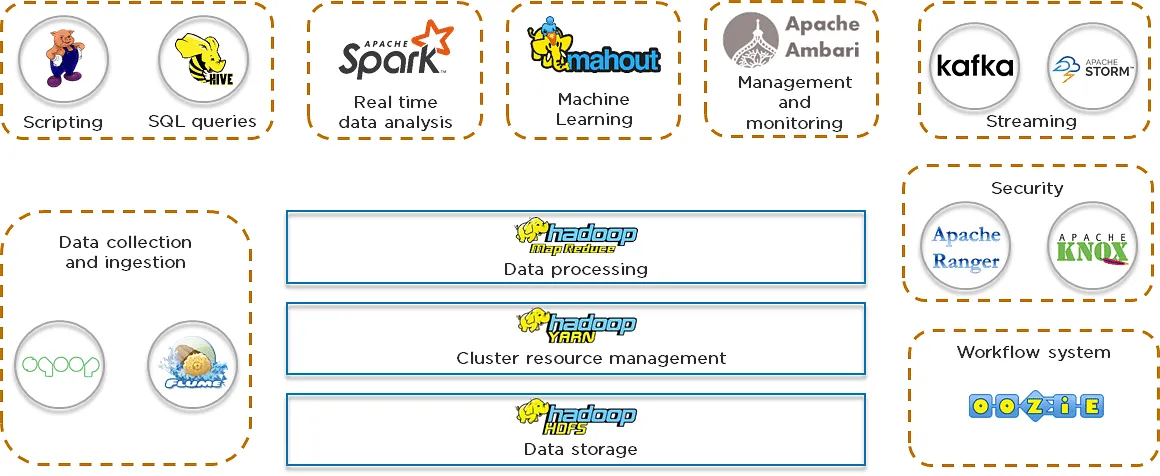
\includegraphics[scale = 0.3]{images/Environment.png}
    \caption{Hadoop Environment}
\end{figure}
\subsection{HDFS}
\subsubsection{Introduction}
Hadoop Distributed File System (HDFS) is a distributed file system that provides reliable and scalable storage for large data sets. It is the primary storage system used in Hadoop environments, and it is designed to store and manage large files across multiple nodes in a cluster. 
\subsubsection{Architecture}
\begin{figure}[h!]
    \centering
    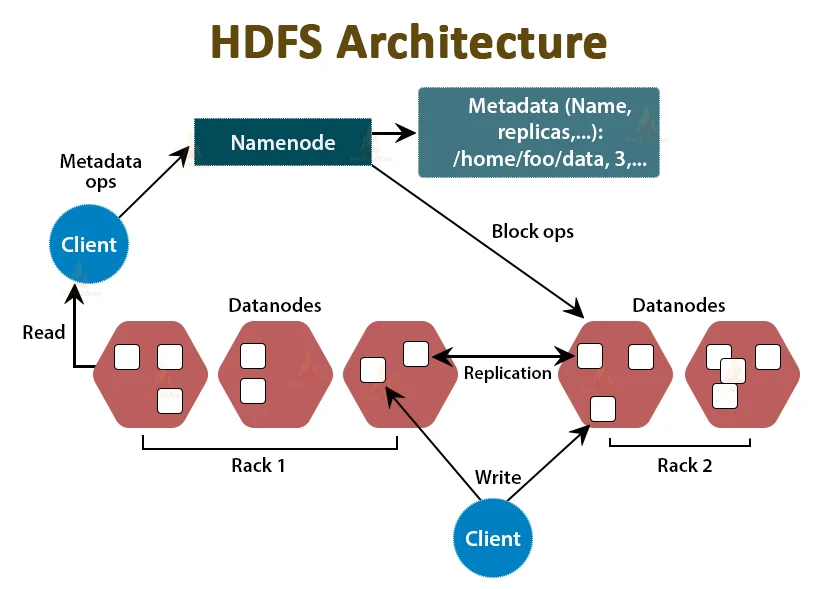
\includegraphics[scale = 0.3]{images/HDFS_Architecture.png}
    \caption{HDFS Architecture}
\end{figure}
HDFS uses a master-slave architecture, where one
node in the cluster acts as the NameNode, which manages the file system namespace and regulates access to files, and multiple nodes act as DataNodes,which store the actual data. The NameNode stores metadata about the files, such as file names, permissions, and the location of data blocks in the cluster. Data is stored in HDFS as blocks, which are typically 128 MB or 256 MB in size. The blocks are replicated across multiple DataNodes in the cluster to provide fault tolerance and ensure data availability even if some nodes fail. The replication factor, or the number of replicas for each block, can be configured based on the desired level of fault tolerance and data redundancy. 
\subsubsection{Uses}
HDFS supports parallel processing of large data sets using the MapReduce, which divides the data into smaller chunks and processes them in parallel across
multiple nodes in the cluster. It is optimized for sequential reads and writes of large files and is designed to handle data-intensive workloads. It is used in various industries, including finance, healthcare, retail, and social media, where the processing and analysis of large data sets are required to gain insights and make informed decisions.
\subsection{YARN}
\subsubsection{Introduction}
YARN (Yet Another Resource Negotiator) is an open-source framework developed by Apache. It is used to manage resources in a Hadoop cluster. It is a central component of Hadoop 2.0 and higher versions. It enables the processing of data with varied processing patterns such as interactive, batch, and real-time processing.
\subsubsection{Architecture}
\begin{figure}[h!]
    \centering
    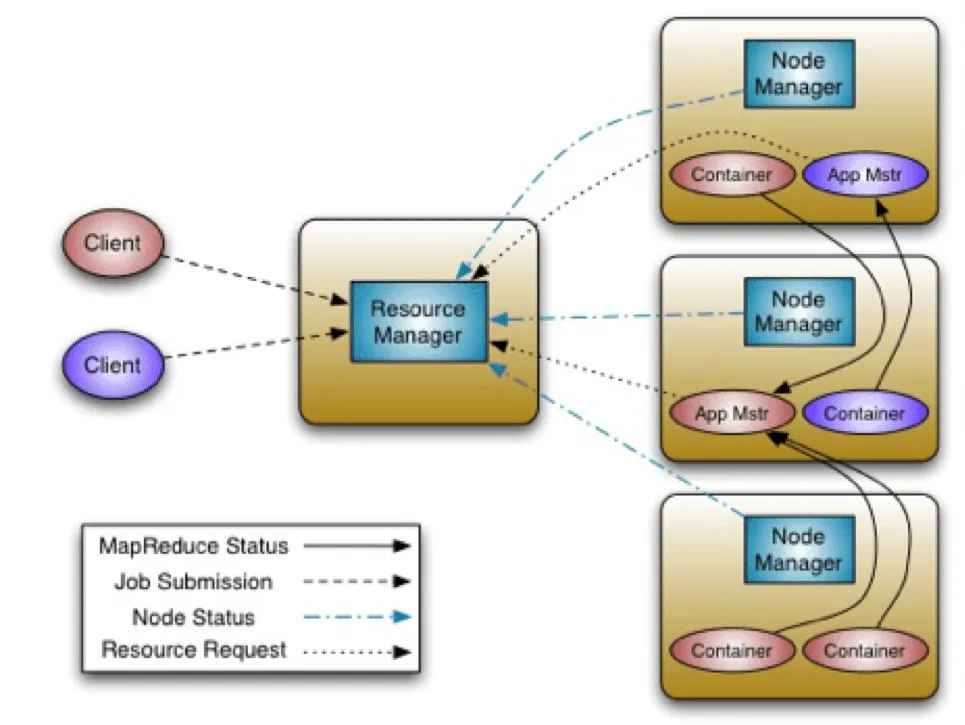
\includegraphics[scale = 0.3]{images/YARN.png}
    \caption{Architecture of YARN}
\end{figure}
YARN consists of two major components: the Resource Manager and the Node Manager. The Resource Manager manages the allocation of resources to various applications running on the cluster, while the Node Manager manages the resources on each individual node. The Resource Manager receives resource requests from clients and allocates the resources to various applications running on the cluster. It also monitors the status of each application and handles failures by reallocating resources or restarting failed components. The Node Manager runs on each node in the cluster and is responsible for managing resources such as memory, CPU, and disk on that node. It communicates with the Resource Manager to request resources and report the status of the resources it is managing.

\subsubsection{Uses}
YARN is used for a variety of big data processing applications, including batch processing, interactive querying, and real-time stream processing. It allows different applications to run on the same cluster, which increases cluster utilization and reduces the cost of managing multiple clusters for different applications. It enables data processing frameworks such as Apache Spark, and Apache HBase to run on the Hadoop cluster, which makes it easy to build complex data processing pipelines. YARN also supports multiple
programming languages such as Java, Python, and R, which makes it easy to develop and deploy applications on the cluster.

\subsection{MapReduce}
\subsubsection{Introduction}
MapReduce is a programming model and software framework for processing and generating large-scale datasets in a parallel and distributed manner. It was
developed by Google and is now widely used in the Hadoop ecosystem for big data processing. The basic idea behind MapReduce is to break down large datasets into smaller chunks and distribute them across a cluster of computers for parallel
processing.
\subsubsection{Architecture}
MapReduce architecture consists of two parts: the Map phase and the Reduce phase. 
\begin{figure}[h!]
    \centering
    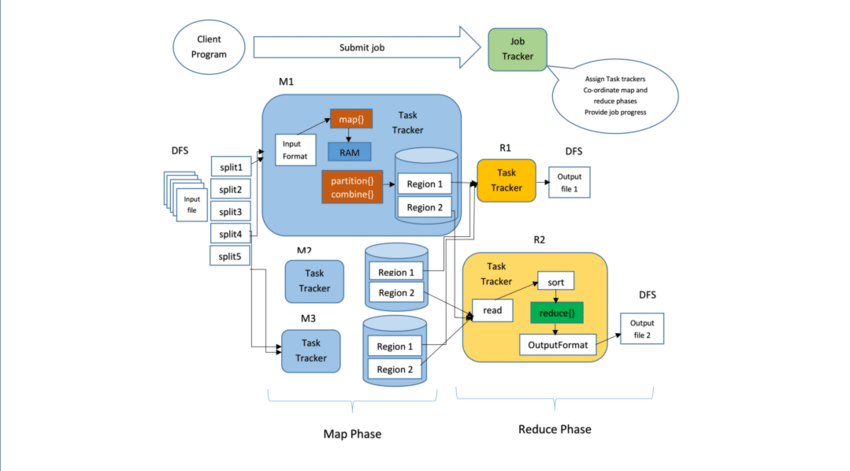
\includegraphics[scale =  0.4]{images/MapReduce.png}
    \caption{Architecture of MapReduce}
\end{figure}
In the Map phase, data is divided into smaller chunks and processed in parallel across multiple nodes in a cluster. Each node runs a Map function that processes the data and produces intermediate key-value pairs. The intermediate data is then shuffled and sorted to group data with the same key, which is sent to the Reduce phase.

In the Reduce phase, the intermediate key-value pairs are processed by a Reduce function that aggregates the data and produces the final output. The output can be stored in a file system or passed on to another MapReduce job for further processing.

The MapReduce framework also includes a JobTracker and TaskTracker. The JobTracker schedules MapReduce jobs and assigns tasks to TaskTrackers running on individual nodes in the cluster. The TaskTrackers run the Map and Reduce functions and report their progress to the JobTracker.
\subsubsection{Uses}
MapReduce is widely used for processing large-scale datasets in various industries for a variety of tasks, such as data cleaning, data transformation, data aggregation, and data analysis. It is particularly useful for processing unstructured and semi-structured data, such as text and log files. It can also be used for processing structured data, such as databases, by converting the data into a format that can be processed by MapReduce.
MapReduce is used in many big data processing frameworks, such as Hadoop and Spark. MapReduce allows developers to write code that can be easily parallelized and run on a cluster of computers, making it a powerful tool for processing big data.

\subsection{Hbase}
\subsubsection{Introduction}
Apache HBase is a column-oriented, distributed, NoSQL database that is designed to store and manage large amounts of structured data. It is built on top of the Hadoop Distributed File System (HDFS) and provides low-latency access to data and is scalable and fault-tolerant.
\subsubsection{Architecture}
\begin{figure}[h!]
    \centering
    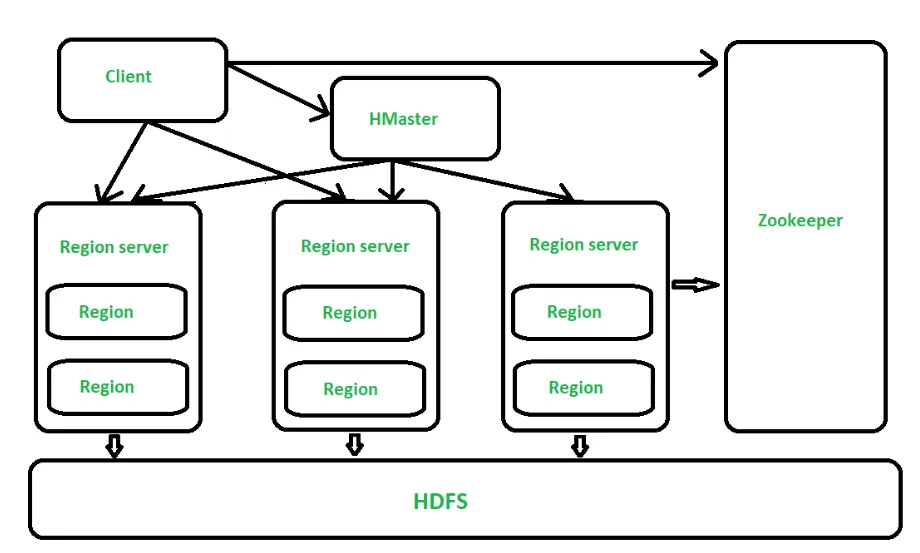
\includegraphics[scale = 0.35]{images/Hbase.png}
    \caption{Hbase architecture}
\end{figure}
HBase architecture consists of four main components: the HMaster, RegionServers, ZooKeeper, and clients. The HMaster is responsible for managing the cluster and assigning regions to RegionServers. The RegionServers are responsible for serving data to clients and managing the regions they are responsible for. ZooKeeper is used for coordination and synchronization between the HMaster and RegionServers.

Data in HBase is organized into tables, which consist of rows and columns. Each table is divided into regions, which are distributed across multiple RegionServers. Data is stored in column families, which are collections of columns. Each column family can have multiple columns, and columns are identified by a column qualifier.

\subsubsection{Uses}
HBase is particularly useful for storing data that requires low-latency access and high availability, such as user profiles, weblogs, and sensor data. It can be used for a variety of use cases, such as real-time analytics, time-series data storage, and online transaction processing (OLTP). It is also used in conjunction with other big data processing frameworks, such as Hadoop and Spark, to provide a complete data processing and management solution.
\subsection{Pig}
\subsubsection{Introduction}
Hadoop Pig is a high-level scripting language platform that is designed to simplify the analysis and processing of large datasets stored in Hadoop. It was developed by Yahoo! and is now an open-source project maintained by the Apache Software Foundation.
\subsubsection{Architecture}
The architecture of Hadoop Pig consists of two main components: the Pig Latin language and the Pig execution environment. 
\begin{figure}[h!]
    \centering
    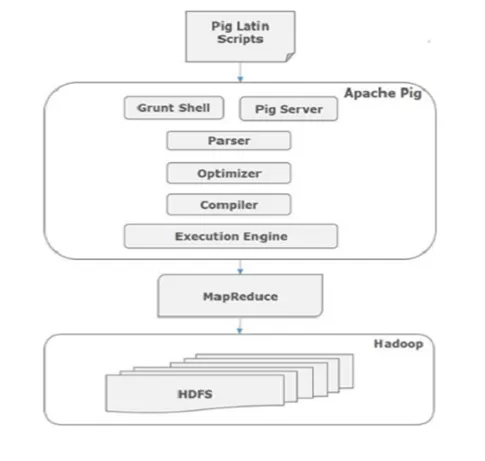
\includegraphics[scale = 0.4]{images/pig.png}
    \caption{Hadoop Pig}
\end{figure}

Pig Latin is a data flow language that provides a SQL-like syntax for expressing data transformations, and the Pig execution environment is a runtime engine that executes Pig Latin scripts on Hadoop clusters. Pig execution environment has following main components : 
\begin{itemize}
    \item Parser
    \item Optimizer
    \item Compiler
    \item Execution Engine
\end{itemize}
\subsubsection{Uses}
Hadoop Pig is commonly used for processing and analyzing large datasets. Its uses include data transformation, data analysis, data processing and data integration. It is an essemtial component in Hadoop ecosystem.
\subsection{Hive}
\subsubsection{Introduction}
Hadoop Hive is a data warehouse system used for large-scale data analysis and querying. It facilitates querying and data analysis of large datasets stored in Hadoop file system. HiveQL is used to analyze structured and semi-structured data, including log files, social media data, and other types of data stored in Hadoop. Hadoop Hive supports several other data analysis languages, including Pig Latin and Java. It also integrates with other Hadoop ecosystem tools, such as Apache Spark and Apache Kafka.
\subsubsection{Architecture}
\begin{figure}[h!]
    \centering
    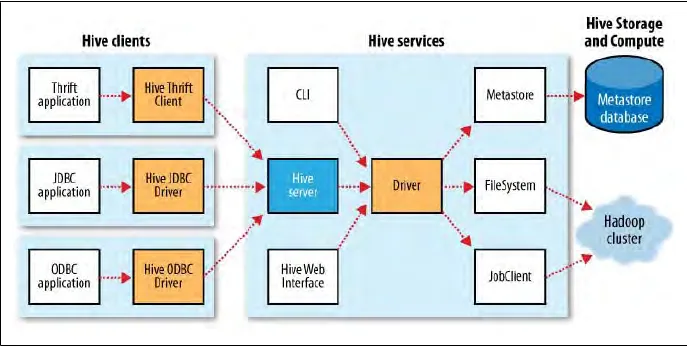
\includegraphics[scale = 0.5]{images/Hive.png}
    \caption{Hadoop Hive}
\end{figure}
Hadoop Hive architecture consists of three main components:
\begin{itemize}
    \item {\bfseries Hive clients}
    These are the applications that connect to the Hive server to submit queries and retrieve results.
    \item {\bfseries Hive server}
    This is the component that receives and manages queries from clients. It also communicates with other Hadoop components to execute queries and fetch data.
    \item {\bfseries HDFS}
\end{itemize}
\subsubsection{Uses}
Hadoop Hive is used for large-scale data analysis and querying. It allows users to write SQL-like queries, known as HiveQL, which are translated into MapReduce jobs by the Hive server. HiveQL is used to analyze structured and semi-structured data, including log files, social media data, and other types of data stored in Hadoop.

\section{Data flow}
In Hadoop, dataflow refers to the process of moving data through various stages of a data processing pipeline. Hadoop is designed to handle large volumes of data, and the dataflow in Hadoop is optimized for processing this data in a distributed and parallel manner. The dataflow in Hadoop is a complex process that involves the storage of data in HDFS and its processing using various Hadoop ecosystem tools.

The data is stored in Hadoop Distributed File System (HDFS). The files are then divided into smaller chunks and distributed across a cluster of nodes. Each node processes the data in parallel, and the results are merged to produce the final output. This distributed processing model allows Hadoop to handle large volumes of data quickly and efficiently.

The dataflow in Hadoop typically consists of following stages :
\begin{enumerate}
    \item {\bfseries Collection and Ingestion : \\}
    The first stage in the dataflow is the collection and ingestion of data into the Hadoop cluster. This data can come from various sources such as logs, sensors, or databases. Hadoop provides various tools for ingesting data, including Flume and Sqoop.
    \item {\bfseries Storage : \\}
    Once the data is ingested, it is stored in the Hadoop Distributed File System (HDFS). 
    \item {\bfseries Processing : \\}
    The next stage in the dataflow is the processing of the data. Hadoop provides a distributed processing framework called MapReduce for this purpose.
    \item {\bfseries Analysis : \\}
    After processing, the data is ready for analysis. Hadoop provides various tools for analyzing data, including Hive, Pig, and Spark.
    \item {\bfseries Visualization : \\}
    The final stage in the dataflow is the visualization of the data. Hadoop provides tools for visualizing data, including Hue and Zeppelin.
\end{enumerate}
The dataflow in Hadoop is designed to be scalable, fault-tolerant, and highly available, making it an ideal platform for processing and analyzing large volumes of data.
\begin{figure}[h!]
    \centering
    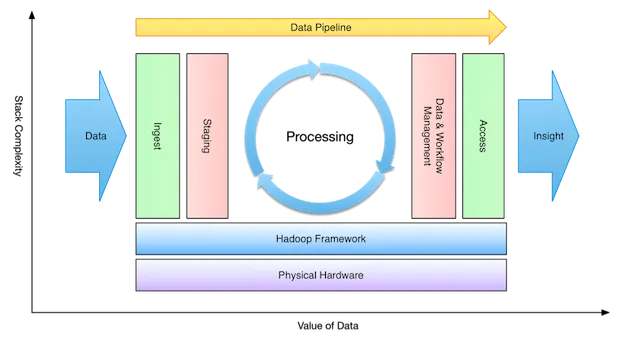
\includegraphics[scale = 0.7]{images/Dataflow.png}
    \caption{Dataflow in Hadoop}
\end{figure}
\section{Hadoop I/O}
Hadoop I/O (Input/Output) refers to the way Hadoop reads and writes data to and from its file system, HDFS. It is a crucial component of the Hadoop ecosystem that provides a set of APIs for reading and writing data in Hadoop. It is optimized for handling large datasets in parallel and distributed manner, which is necessary for the big data processing that Hadoop is designed for.

Hadoop I/O contains several classes and interfaces that enable data processing in Hadoop. One such class is the InputFormat class, which defines how input data is split and read in MapReduce jobs. The RecordReader class reads and decodes the input data, and the OutputFormat class defines how output data is written to the HDFS. The RecordWriter class writes the output data in a specified format that can be read by other Hadoop ecosystem tools. Hadoop I/O also provides support for custom input and output formats, which allows users to define their own file formats for reading and writing data in Hadoop. This flexibility allows users to work with data in a way that is specific to their needs.

Hadoop I/O provides several APIs that developers can use to interact with HDFS:
\begin{enumerate}
    \item Hadoop FileSystem API : \\
    This API provides low-level access to HDFS and allows developers to perform basic file operations like reading, writing, and deleting files.
    \item Hadoop MapReduce API: \\
    This API provides a framework for distributed data processing, where data is read from HDFS, processed in parallel across a cluster of machines, and then written back to HDFS.
    \item Hadoop Streaming API: \\
    This API allows developers to write MapReduce jobs in any language that can read from and write to standard input/output streams, such as Python, Ruby, and Perl.
    \item Hadoop Distributed Cache API: \\
    This API provides a mechanism for distributing read-only data, such as lookup tables, to all nodes in a Hadoop cluster for use in MapReduce jobs.
\end{enumerate}

In addition to these APIs, Hadoop also provides several libraries and tools for working with Hadoop I/O, including Apache Avro, Apache Parquet, and Apache ORC for efficient serialization and deserialization of data, and Apache Flume and Apache Sqoop for data ingestion. Overall, Hadoop I/O is a critical component of the Hadoop ecosystem that provides a unified interface for reading and writing data in Hadoop. It offers support for various file formats as well as compression and serialization features, which make it easier for users to work with large datasets stored in HDFS.

\section{Query Languages for Hadoop}
Hadoop is a distributed computing platform that allows processing of large datasets across multiple servers in a cluster. There are several query languages available for Hadoop, each with its own strengths and use cases.
Here are some of the popular query languages for Hadoop:
\subsection{HiveQL}
Hadoop Hive uses a SQL-like language called HiveQL for querying and analyzing data. It is used to process structured and semi-structured data stored in Hadoop's distributed file system (HDFS). It provides a familiar high-level SQL-like interface and supports many SQL features like joins, group-by, and aggregation functions. HiveQL is translated into MapReduce jobs by the Hive server, making it possible to analyze large datasets quickly and efficiently.
\subsection{Apache Drill}
Apache Drill is a schema-free SQL query engine for Hadoop and NoSQL. It allows users to query a variety of data stores, including Hadoop Distributed File System (HDFS), NoSQL databases, and cloud storage services, using standard SQL queries. Apache Drill is designed to handle complex queries on large datasets, making it a good choice for data exploration and analysis.
\subsection{Apache Phoenix}
Apache Phoenix is a SQL query engine for HBase, a distributed NoSQL database in Hadoop. It provides a JDBC driver and a SQL-like syntax for querying data stored in HBase. Apache Phoenix is optimized for low-latency queries on large datasets, making it a good choice for applications that require real-time data access.
\subsection{Hadoop Impala}
Hadoop Impala is an SQL query engine designed specifically for Hadoop. It allows users to query data stored in HDFS using standard SQL queries, and provides high-performance, low-latency access to large datasets. It can handle complex queries on large datasets quickly and efficiently. It is designed for interactive data analysis, making it a good choice for applications that require real-time data access.
\subsection{Apache Spark SQL}
Apache Spark SQL is a SQL query engine in Apache Spark that provides a programming interface to work with structured and semi-structured data. It supports both SQL and Dataframe APIs for querying data stored in Hadoop. It provides a powerful and flexible interface for querying and manipulating data in Spark. It allows users to query data stored in Hadoop, NoSQL databases, and other data sources using standard SQL queries. It is designed to handle complex queries on large datasets, making it a good choice for applications that require real-time data access.
\subsection{Pig Latin}
Pig Latin is a high-level data flow language that is used to process both structured and unstructured data stored in Hadoop. It provides a simple and flexible syntax that allows users to write complex data processing workflows with ease.
\subsection{Hbase Query Language}
HBase is a NoSQL database that is built on top of Hadoop's distributed file system. HQL is a query language used to interact with HBase tables. It provides a SQL-like syntax for querying data and supports a variety of filters, scans, and aggregations.

The choice of query language for Hadoop depends on the specific use case and requirements of the application.
\section{Hadoop and Amazon Cloud}
Hadoop is an open-source distributed computing platform that can be used to store, process and analyze large volumes of data. Amazon Web Services (AWS) is a cloud computing service provider that offers various services, including Hadoop-based services.

Amazon Web Services (AWS) provides a number of services that integrate with Hadoop, including Amazon Elastic MapReduce (EMR), Amazon S3, and Amazon DynamoDB.AWS provides a managed Hadoop service called Amazon EMR (Elastic MapReduce). EMR simplifies the deployment and management of Hadoop clusters on AWS by providing pre-configured Amazon Machine Images (AMIs) and an easy-to-use web interface for managing and scaling the clusters. EMR also supports other big data frameworks, such as Apache Spark and Apache Hive. In addition to EMR, AWS offers other services that can be used together with Hadoop to build a cost-effective big data solution. For example, Amazon S3 (Simple Storage Service) can be used as a data store for Hadoop clusters, and Amazon Redshift can be used to build data warehouses for analytics. Amazon DynamoDB is a NoSQL database service that can be used to store and retrieve data for use with Hadoop and other big data tools. Together, these services provide a comprehensive solution for big data processing and analysis in the cloud.

Overall, using Hadoop on AWS can provide many benefits, such as reduced infrastructure management overheads, faster deployment times, and more flexibility and scalability.

  
\section{Current State of Hadoop}
Hadoop in big data is no longer the only option for big data processing and storage. In recent years, cloud-based solutions such as Amazon Web Services (AWS) and Microsoft Azure have become increasingly popular for big data processing and storage, offering a range of managed services that make it easier and more cost-effective to manage big data workloads. These cloud-based solutions often provide integrations with Hadoop-based technologies, such as Apache Spark and Apache Hive, allowing organizations to take advantage of Hadoop's strengths while leveraging the benefits of the cloud. Additionally, newer technologies such as Apache Kafka, Apache Flink, and Apache Beam have emerged, providing real-time data streaming and processing capabilities that are complementary to Hadoop. These technologies enable organizations to process and analyze data in real-time, allowing for faster and more efficient decision-making. Despite these new developments, Hadoop is still widely used in many industries. Hadoop's strengths in distributed processing, data storage, and data analysis make it a powerful tool for big data processing and storage.

Overall, the current state of Hadoop in big data is that it is still relevant, but it is now part of a larger ecosystem of tools and technologies that enable organizations to process and analyze big data in a variety of ways. Together, these services along with Hadoop provide a comprehensive solution for big data processing and analysis in the cloud.
\end{document}